\documentclass{article}
\usepackage[utf8]{inputenc}
\usepackage{pgfplots}
\usepackage{fancyhdr}
\usepackage{enumitem}
\usepackage{tikz}
\usepackage{xparse}
\usepackage{siunitx}

\pgfplotsset{width=10cm,compat=1.9}

\pagestyle{fancy}
\fancyhf{}
\lhead{Steven Glasford}
\chead{Homework 1.4}
\rhead{Page \thepage}

\title{Homework 1.4}
\author{Steven Glasford}
\date{\parbox{\linewidth}{\centering%
    \today\endgraf\medskip
    Math-451-M001}}
\newcommand{\rpm}{\sbox0{$1$}\sbox2{$\scriptstyle\pm$}
  \raise\dimexpr(\ht0-\ht2)/2\relax\box2 }
  
\newlist{steps}{enumerate}{1}
\setlist[steps, 1]{label = Step \arabic*:}
\ExplSyntaxOn
\newcommand*{\prlen}[1]{%
   % round to 1 digit:
    \pgfmathparse{round(10)/10.0}%
    %\pgfkeys{/pgf/number format/precision=1}
    %\pgfmathresult
    \pgfmathprintnumber[fixed, precision=2]{\pgfmathresult}
}
\ExplSyntaxOff


\begin{document}

\maketitle

I choose to do problems 3 and 9 from the options of 3, 4, 5 and 9.

\section{Problem 3}

\begin{enumerate}[label=\alph*]
    \item 
    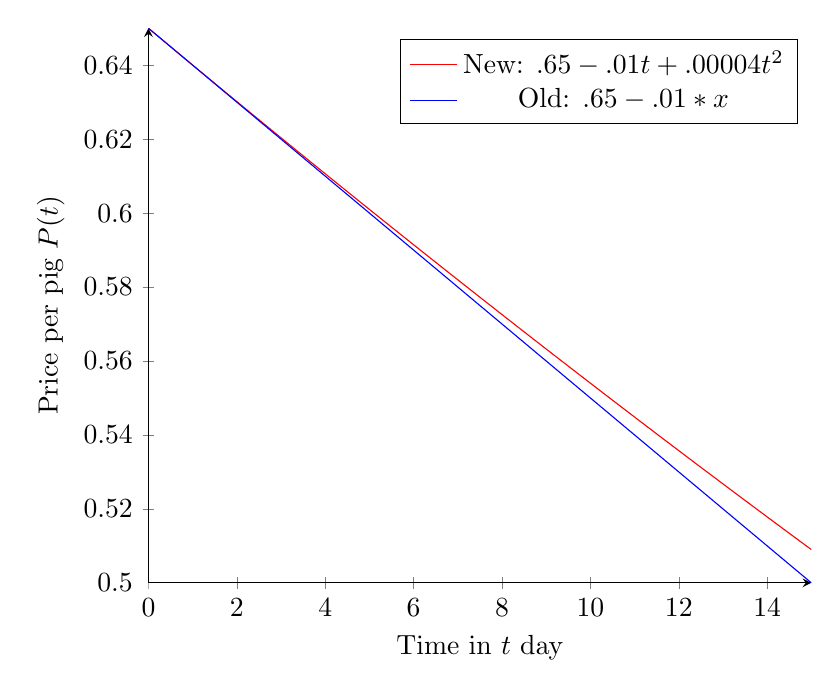
\begin{tikzpicture}
        \begin{axis}[
            axis lines = left,
            xlabel = Time in $t$ day,
            ylabel = Price per pig $P(t)$,
        ]
        \addplot [
            domain=0:15,
            samples=100,
            color=red,
        ]{.65 - .01*x + .00004*x^2};
        \addlegendentry{New: $.65-.01t+.00004t^2$}
        
        \addplot[
            domain=0:15,
            samples=100,
            color=blue,
        ]{.65-.01*x};
        \addlegendentry{Old: $.65-.01*x$}
        
        \end{axis}
    \end{tikzpicture}
    The graph above shows the price per pig using both the old linear model (blue) and the newer model (the red line). The red line is more accurate to the actual price per pig in real life. But as is obvious in the graph the values for the old equation are very similar to the more accurate model within the appropriate time domain.
    \item
        \begin{center}
            \begin{tabular}{ |c|c|c| } 
            \hline 
            Variables & Constants & Assumptions \\
            \hline
            $t$ - Time (Days) & $w_0 = 200$ initial weight (pounds) & $w=w_0+5t$ \\
            $f$ - profit (in dollars) &  & $p=.65-.01t+.00004t^2$ \\ 
            $w$ - Weight (pounds) && $c=.45t$ \\ 
            $p$ - Price per pound && $r=p*w$\\
            $c$ - cost (in dollars) && $f=r-c$\\
            $r$ - Revenue (in dollars) &&\\
            \hline
            \end{tabular}
        \end{center}
        If we want to maximize $f(t)$ then we should try to add all of the assumptions into a single equation, this way all of the assumptions are considered. We will try to use $t$ as the isolating factor. If $$f=r-c$$ \parbox{\linewidth}{\centering% 
            $r=pw$ \hspace*{3cm} $c=.45t$ \endgraf \bigskip 
            $f=pw-.45t$ \endgraf\bigskip
            $p=.65-.01t$ \hspace*{3cm}
            $w=w_0+5*t$ \endgraf \bigskip
            $f=(.65-.01t+.00004t^2)(w_0+5t)-.45t$ \endgraf\bigskip
            $w_0=200$ \endgraf \bigskip
            $f=(.65-.01t+.00004t^2)(200+5t)-.45t$ \endgraf\bigskip
        } 
        Which simplifies to:$$f(t)=.0002t^3-.042t^2+.8t+130$$
        Now we need to take the derivative of $f(t)$ and find where it is equal to zero. $$\frac{df}{dt}=\frac{3t^2}{5000}-\frac{21t}{250}+\frac{4}{5}$$
        
        \begin{tikzpicture}
        \begin{axis}[
            axis lines = left,
            xlabel = Time in $t$ day,
            ylabel = $y$,
        ]
        
        \addplot[
            domain=0:20,
            samples=100,
            color=blue,
        ]{(3*x^2-420*x+4000)/5000};
        \addlegendentry{$\frac{df}{dt}$}
        \draw[ultra thin] (axis cs:\pgfkeysvalueof{/pgfplots/xmin},0) -- (axis cs:\pgfkeysvalueof{/pgfplots/xmax},0);
        \end{axis}
        
    \end{tikzpicture}
    \endgraf
    Using the quadratic equation we try to determine the extreme somewhere between 8 and 14, as that point will be a maximum, this is known since the derivative is a quadratic and that point the derivative goes from positive to negative, indicating a maxima. The other root would in turn be a minima.
    $$\frac{df}{dt}=0=\frac{3t^2-420t+4000}{5000}$$ $$t=\frac{10(21+\sqrt{321})}{3},\frac{10(21-\sqrt{321})}{3}$$
    $$t \approx \pgfmathparse{(10*(21+321^(1/2)))/3}\pgfmathresult , \pgfmathparse{(10*(21-321^(1/2)))/3}\pgfmathresult $$
    \textbf{Therefore, the best day to sell your pig is at about 10 days.}
    
    \item \underline{Sensitivity analysis}
    \endgraf
    $$p(t)=.65-.01t+.00004t^2$$
    $$f(t)=.0002t^3-.042t^2+.8t+130$$
    $$y=(.65-.01x+xt^2)(200+5x)-.45x$$
    $$y=5rx^3-.05x^2+200rx^2+.8x+130=0$$
    $$\frac{dy}{dx}=15rx^2+400rx-\frac{x}{10}+\frac{4}{5}=0$$
    $$x=\frac{-4000r+1+ 10\sqrt{160000r^2-128r+1/100}}{300r}$$
    $$\frac{dx}{dr}=\frac{-6400r+1+ \sqrt{16000000r^2-12800r+1}}{300r^2\sqrt{16000000r^2-12800r+1}}$$
    \begin{center}
            \begin{tabular}{ |c|c|c| } 
            \hline 
            r & x & $\frac{\Delta x}{\Delta r} * 100$ \\
            \hline
            .00002 & 297.709385518&
            %\pgfkeys{/pgf/fpu} \pgfmathparse{}\pgfmathresult
            %\edef\tmp{\pgfmathresult}
            %\pgfmathresult
            %\pgfkeys{/pgf/fpu=false} &
            %1/(-6400*.00004+1+sqrt(16000000*.00004^2-128*.00004+1))/(300*.00004^2*sqrt(16000000*.00004^2-12800*.00004+1))
            %(-6400*r+1+\sqrt{16000000*r^2-128*r+1})/(300*r^2*\sqrt{16000000*r^2-12800r+1})
             
            \\
            .00003 & 185.997481072  & -1117119044.46
            %\pgfmathparse{((-4000*.00003+1+10*(160000*.00003^2-128*.00003+1/100)^(1/2))/(300*.00003)-(-4000*.00002+1+10*(160000*.00002^2-128*.00002+1/100)^(1/2))/(300*.00002))/(.00003-.00002)*100}\pgfmathresult &
            \\
            .00004 &129.721576224&-562759048.485
           % \pgfmathparse{(-4000*.00004+1+10*(160000*.00004^2-128*.00004+1/100)^(1/2))/(300*.00004)}\pgfmathresult &
           % \pgfmathparse{(-4000*.00004+1-10*(160000*.00004^2-128*.00004+1/100)^(1/2))/(300*.00004)}\pgfmathresult &
           % \pgfmathparse{((-4000*.00004+1+10*(160000*.00004^2-128*.00004+1/100)^(1/2))/(300*.00004)-(-4000*.00003+1+10*(160000*.00003^2-128*.00003+1/100)^(1/2))/(300*.00003))/(.00004-.00003)*100}\pgfmathresult &
           % \pgfmathparse{((-4000*.00004+1-10*(160000*.00004^2-128*.00004+1/100)^(1/2))/(300*.00004)-(-4000*.00003+1-10*(160000*.00003^2-128*.00003+1/100)^(1/2))/(300*.00003))/(.00004-.00003)*100}\pgfmathresult
            \\
            .00005 & 95.4970354689 &-342245407.55
            %\pgfmathparse{(-4000*.00005+1+10*(160000*.00005^2-128*.00005+1/100)^(1/2))/(300*.00005)}\pgfmathresult &
           % \pgfmathparse{(-4000*.00005+1-10*(160000*.00005^2-128*.00005+1/100)^(1/2))/(300*.00005)}\pgfmathresult &
           % \pgfmathparse{((-4000*.00005+1+10*(160000*.00005^2-128*.00005+1/100)^(1/2))/(300*.00005)-(-4000*.00004+1+10*(160000*.00004^2-128*.00004+1/100)^(1/2))/(300*.00004))/(.00005-.00004)*100}\pgfmathresult&
           % \pgfmathparse{((-4000*.00005+1-10*(160000*.00005^2-128*.00005+1/100)^(1/2))/(300*.00005)-(-4000*.00004+1-10*(160000*.00004^2-128*.00004+1/100)^(1/2))/(300*.00004))/(.00005-.00004)*100}\pgfmathresult
            \\
            .00006 &72.1191645491&-233778709.199
            %\pgfmathparse{(-4000*.00006+1+10*(160000*.00006^2-128*.00006+1/100)^(1/2))/(300*.00006)}\pgfmathresult &
           % \pgfmathparse{(-4000*.00006+1-10*(160000*.00006^2-128*.00006+1/100)^(1/2))/(300*.00006)}\pgfmathresult &
           % \pgfmathparse{((-4000*.00006+1+10*(160000*.00006^2-128*.00006+1/100)^(1/2))/(300*.00006)-(-4000*.00005+1+10*(160000*.00005^2-128*.00005+1/100)^(1/2))/(300*.00005))/(.00006-.00005)*100}\pgfmathresult&
           % \pgfmathparse{((-4000*.00006+1-10*(160000*.00006^2-128*.00006+1/100)^(1/2))/(300*.00006)-(-4000*.00005+1-10*(160000*.00005^2-128*.00005+1/100)^(1/2))/(300*.00005))/(.00006-.00005)*100}\pgfmathresult
            \\
            \hline
            \end{tabular} 
    \end{center}
    \textbf{Therefore the best sort of sensitivity is somewhere between .00004 and .00005}
    
    
    %% \pgfmathparse{(10*(21-321^(1/2)))/3}\pgfmathresult
    \item The robustness is fairly good since the values obtained from both the linear and the quadratic models are roughly similar.
    
\end{enumerate}

\section{Problem 9}

\begin{enumerate}[label=\alph*]
    \endgraf
    \item\endgraf\bigskip

    
        \begin{steps}
            \endgraf
            \item \emph{Ask the Question, determine variables, constants, assumptions}\endgraf
            \begin{center}
                \begin{tabular}{ |c|c|c|c| } 
                \hline 
                Variables & Constants & Assumptions \\
                \hline
                $s$ - Subscribers & $i_0 = 1.50$ & $f=sp$\\
                $p$ - Subscription price & $s_0=80000$&$s=s_0-50000(p-p_0)$\\
                $f$ - Profits &&$p\geq0$\\
                && $s\geq0$\\
                
            \hline
            \end{tabular}
        \end{center}
            \item \emph{Select the model}\endgraf
            One-variable optimization
            \item \emph{Formulate the model} \endgraf
            $$f=sp$$
            $$s=s_0-50000(p-p_0)$$
            $$f=p(s_0-50000(p-p_0))$$
            \parbox{\linewidth}{\centering% 
            $s_0=80000$ \hspace*{3cm} $p_0=1.50$ \endgraf \bigskip
            }
            $$f=p(80000-50000(p-1.5))$$
            or simplified
            $$f=-50000p^2+155000p$$
            \item \emph{Solve the model}\endgraf
            Find the extrema for f:
            $$\frac{df}{dp}=0=-100000p+155000$$
            $$p=1.55$$
            Determine if 1.55 is a max or min:
            \begin{tikzpicture}
                \begin{axis}[
                axis lines = left,
                xlabel = Price per paper,
            ]
            \addplot [
                domain=0:2,
                samples=100,
                color=red,
            ]{-100000*x+155000};
            \addlegendentry{$\frac{df}{dp}$}
            \draw[ultra thin] (axis cs:\pgfkeysvalueof{/pgfplots/xmin},0) -- (axis cs:\pgfkeysvalueof{/pgfplots/xmax},0);
        \end{axis}
    \end{tikzpicture}
        Since the derivative of $f$ is going from positive to negative at the point 1.55, \textbf{$p=1.55$ is a Maximum.}\bigskip
            \item \emph{Answer the question}\endgraf
            The best price to sell the newspaper is \$1.55 for a total of \$$120125$ per week, and a total of $77500$ subscribers.
        \end{steps}
    
    %% \pgfmathparse{(10*(21-321^(1/2)))/3}\pgfmathresult
    
    \item \endgraf \bigskip
        \emph{What if the newspaper lost a different number of subscribers, other than 5000?}
        $$f=p(80000-r*10(p-1.5))$$
        $$\frac{df}{dp}=0=-20rp+15r+80000$$
        $$p=\frac{80000+15r}{20r}$$
        replace $p$ in the $f$ equation:
        $$f=\frac{80000+15r}{20r}\left(80000-10r\left(\frac{80000+15r}{20r}-1.5\right)\right)$$
        Which doesn't really simplify down to anything worth mentioning.
        \begin{center}
                \begin{tabular}{ |c|c| } 
                \hline 
                Lost Subscribers ($r$) & Max Profit \\
                \hline
                3000 &\$130208.33\\
                4000 &\$122500.00\\
                5000 &\$120125.00\\
                6000 &\$120416.67\\
                7000 &\$122232.14\\
                
                
            \hline
        \end{tabular}
    \end{center}
    \item
    $$f=\frac{80000+15r}{20r}\left(80000-10r\left(\frac{80000+15r}{20r}-1.5\right)\right)$$
    $$\frac{df}{dr}=\frac{45r^2-1280000000}{8r^2}$$
    Sensitivity=$\frac{df}{dr}*\frac{r}{x}=S(p,n)$
    $$S(p,n)=\frac{45n^2-1280000000}{8n^2}\left(n/\left(\left(\frac{80000+15n}{20n}\left(80000-10n\left(\frac{80000+15n}{20n}-1.5\right)\right)\right)\right)\right)$$
    \item \emph{The Newspaper shouldn't need to change its prices.} The price is already near the optimal rate, but the optimal rate is just \$125 more than the basic, which is basically nothing when considering the amount of profit they received.
    
\end{enumerate}


\end{document}